\chapter{Opgaveformulering (MK PO)}

Konstruer et system til vanding af golfbaner. Systemet skal indeholde én Master (Devkit8000) som kontrollerer et netværk af Enheder (PSoC4). Kommunikationen mellem Master og Enhed skal foregå via den serielle kommunikation kaldet SPI. Via denne kommunikation skal Masteren kunne kontrollere de enkelte Enheder, samt indhente log-data fra disse. 
Enheden skal fungere autonomt, når denne er aktiveret. Enheden  er tilkoblet en komponentpakke bestående af fugt- og temperatursensor samt sprinkler med tilhørende pumpe og vandforsyning. Enheden skal således selv styre vanding af trængende områder. En bevægelsessensor skal placeres ved indgangen til hvert golfhul, hvis der registreres bevægelse blokeres en evt. vanding i 30 minutter.  

Figur \ref{fig:systemoversigt} illustrerer ovenstående.  

%SYSTEMOVERBLIK BILLEDE
\begin{figure}[h]
  \centering
    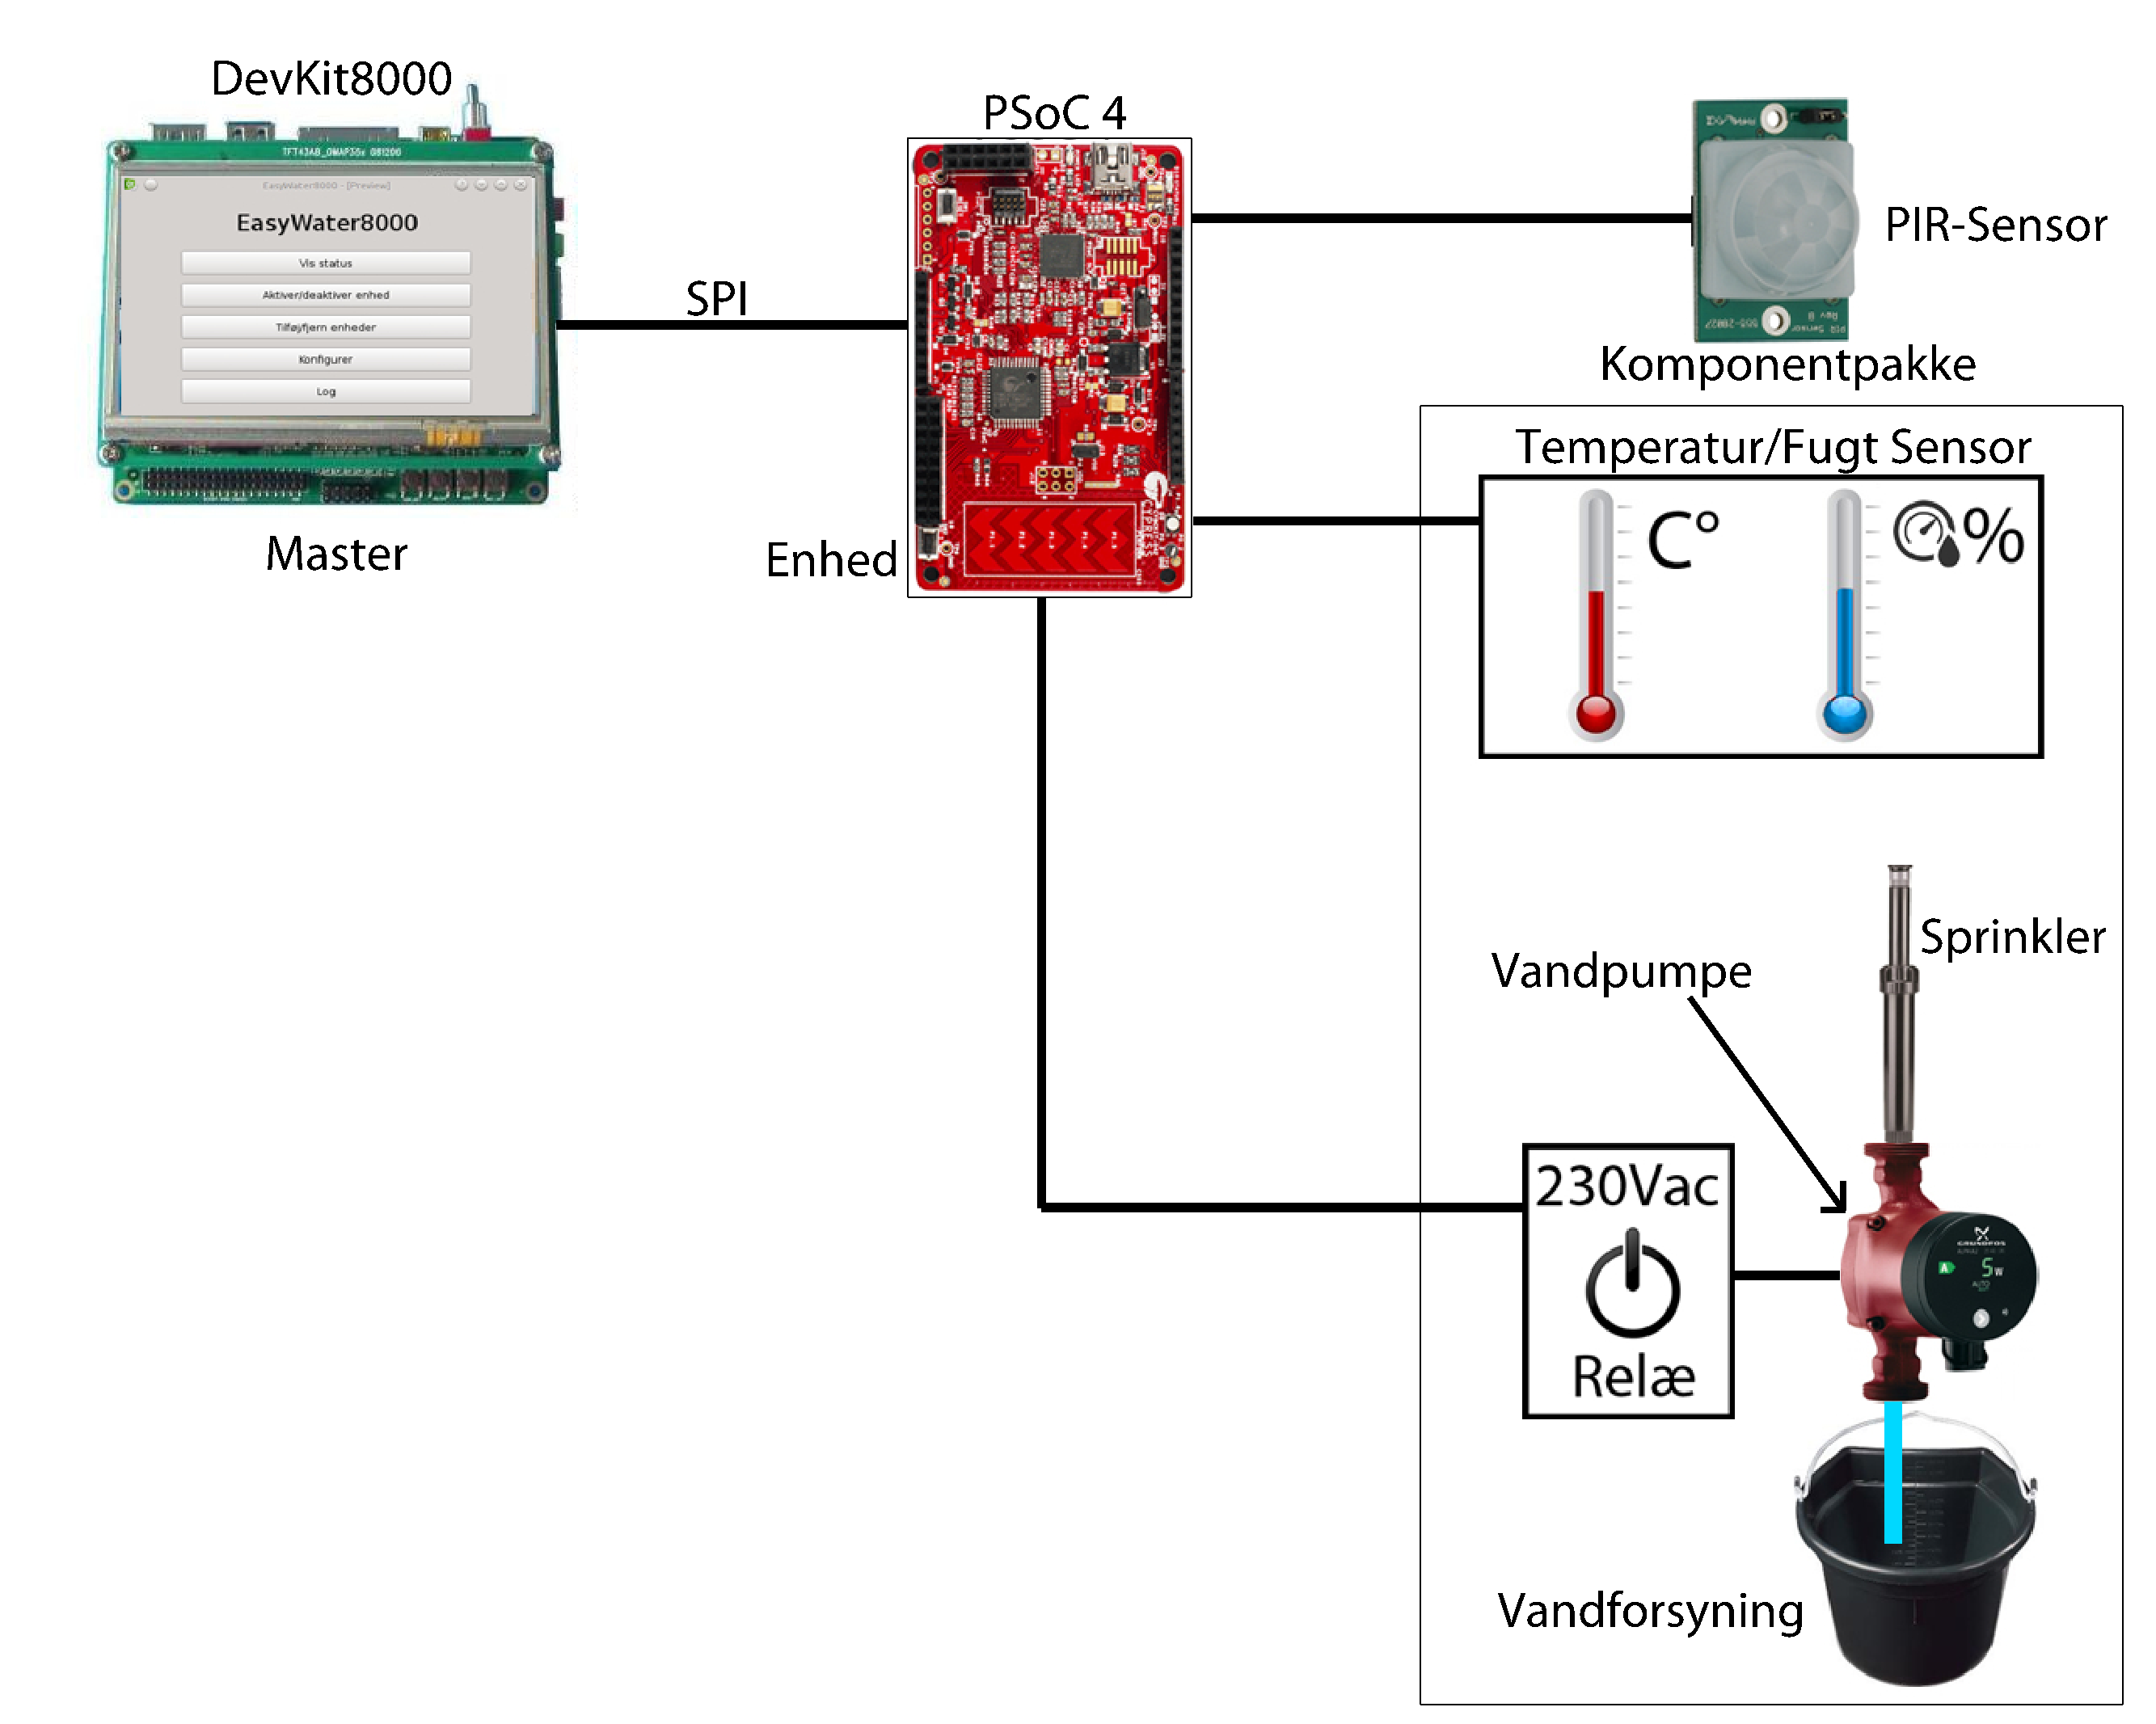
\includegraphics[width=\textwidth]{Billeder/systemoversigt}
    \caption{Systemoversigt}
    \label{fig:systemoversigt}
\end{figure}
